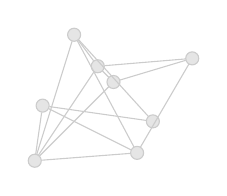
\begin{tikzpicture}
                [   cnode/.style={draw=black,fill=#1,minimum width=3mm,circle},
            rnode/.style={draw=#1!40,fill=#1!20,minimum width=6mm, minimum height=6mm, rectangle},
            gnode/.style={draw=gray!40,fill=gray!20,circle,scale=0.5},
            gline/.style={gray!40}
        ]
        
        
        \node[gnode] (a1) at (0, 0) {};
        \node[gnode] (a2) at (0.8, 1.2) {};
        \node[gnode] (a3) at (0.5, 1.6) {};
        \node[gnode] (a4) at (0.1, 0.7) {};
        \node[gnode] (a5) at (1.5, 0.5) {};
        \node[gnode] (a6) at (1.3, 0.1) {};
        \node[gnode] (a7) at (2, 1.3) {};
        \node[gnode] (a8) at (1, 1) {};
        
        \draw[gline] (a1) -- (a2);
        \draw[gline] (a1) -- (a3);
        \draw[gline] (a1) -- (a8);
        \draw[gline] (a1) -- (a4);
        \draw[gline] (a7) -- (a6);
        \draw[gline] (a7) -- (a2);
        \draw[gline] (a2) -- (a3);
        \draw[gline] (a3) -- (a6);
        \draw[gline] (a4) -- (a6);
        \draw[gline] (a1) -- (a6);
        \draw[gline] (a7) -- (a8);
        \draw[gline] (a4) -- (a5);
        \draw[gline] (a3) -- (a5);
        \draw[gline] (a8) -- (a2);
            \end{tikzpicture}